%%%%%%%%%%%%%%%%%%%%%%%%%%%%%%%%%%%%
% This is the template for submission to ISCA 2016
% The cls file is a modified from  'sig-alternate.cls'
%%%%%%%%%%%%%%%%%%%%%%%%%%%%%%%%%%%%

\documentclass{sig-alternate} 
\usepackage{mathptmx} % This is Times font

\newcommand{\ignore}[1]{}
\usepackage{fancyhdr}
\usepackage[normalem]{ulem}
\usepackage[hyphens]{url}
\usepackage{hyperref}


%%%%%%%%%%%---SETME-----%%%%%%%%%%%%%
\newcommand{\hpcasubmissionnumber}{NaN}
%%%%%%%%%%%%%%%%%%%%%%%%%%%%%%%%%%%%

\fancypagestyle{firstpage}{
  \fancyhf{}
\setlength{\headheight}{50pt}
\renewcommand{\headrulewidth}{0pt}
  \fancyhead[C]{} 
  \pagenumbering{arabic}
}  

%%%%%%%%%%%---SETME-----%%%%%%%%%%%%%
\title{Extract Useful Features for Detecting Transient Faults} 
\author{Zhiqiang Sui, Zhefan Ye, Karthik Desingh}
%%%%%%%%%%%%%%%%%%%%%%%%%%%%%%%%%%%%

\begin{document}
\maketitle
\thispagestyle{firstpage}
\pagestyle{plain}

\begin{abstract}

\end{abstract}

\section{Introduction}
We present 

\begin{figure}[t]
\begin{center}
   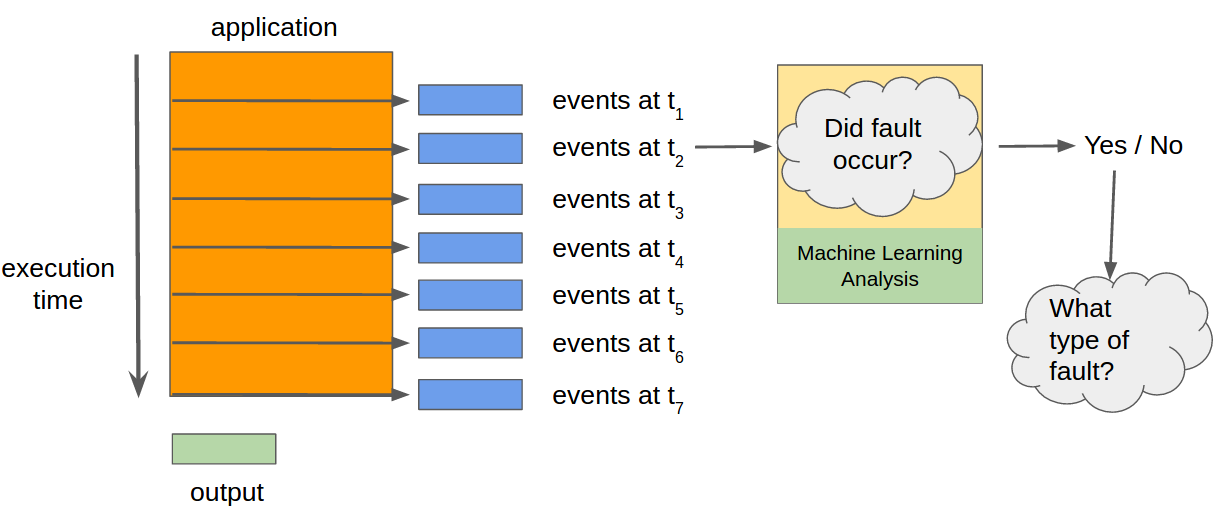
\includegraphics[width=0.95\linewidth]{./figures/teaser.png}
\end{center}
   \caption{Overview}
\label{fig:teaser}
\end{figure}

\section{Related Work}

\section{Approach}
We present

\begin{figure}[t]
\begin{center}
   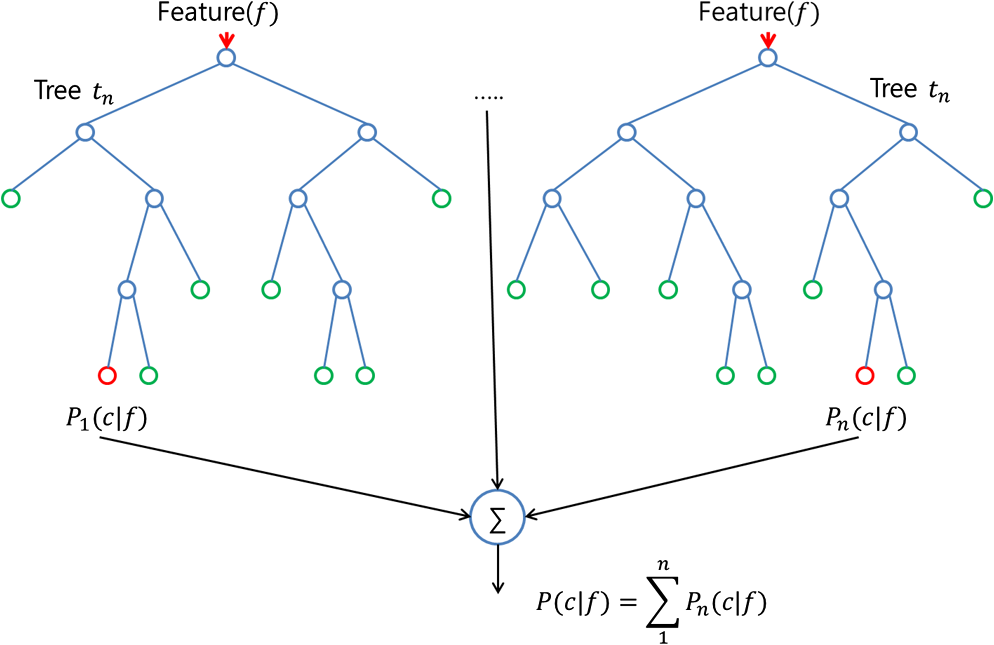
\includegraphics[width=0.95\linewidth]{./figures/rf.png}
\end{center}
   \caption{}
\label{fig:rf}
\end{figure}

\subsection{Pipeline}

\begin{figure*}[t]
\begin{center}
   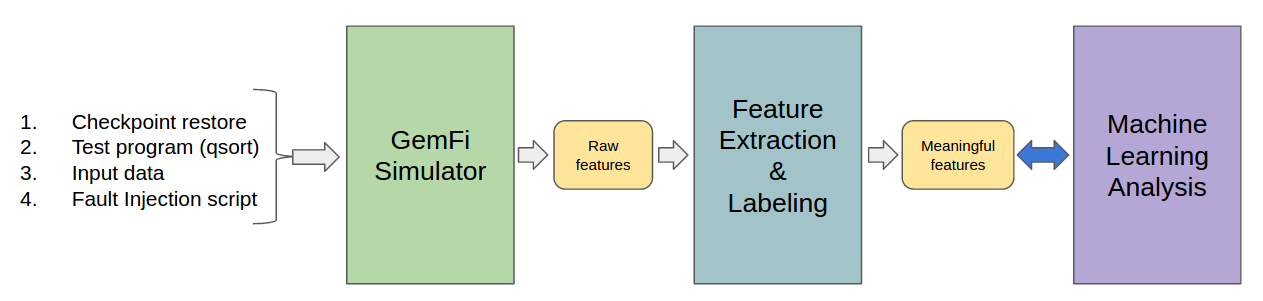
\includegraphics[width=0.95\linewidth]{./figures/pipeline.png}
\end{center}
   \caption{}
\label{fig:pipeline}
\end{figure*}

\subsection{Fault Injection}

\subsection{Feature Extraction}

\begin{figure*}[t]
\begin{center}
   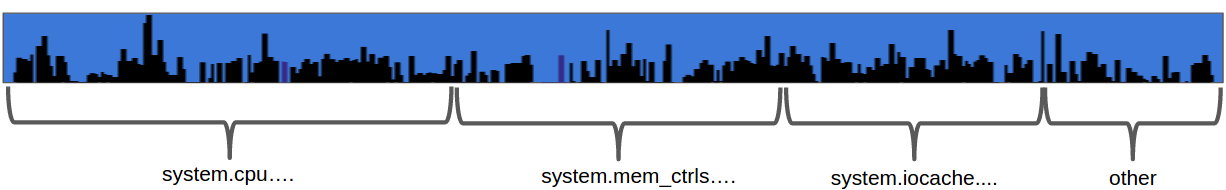
\includegraphics[width=0.95\linewidth]{./figures/feat_dist.png}
\end{center}
   \caption{}
\label{fig:feat-dist}
\end{figure*}

\subsection{Machine Analysis}

\subsubsection{Training and Testing}

\section{Experiment}

\subsection{Same Input All Features}

\begin{figure}[t]
\begin{center}
   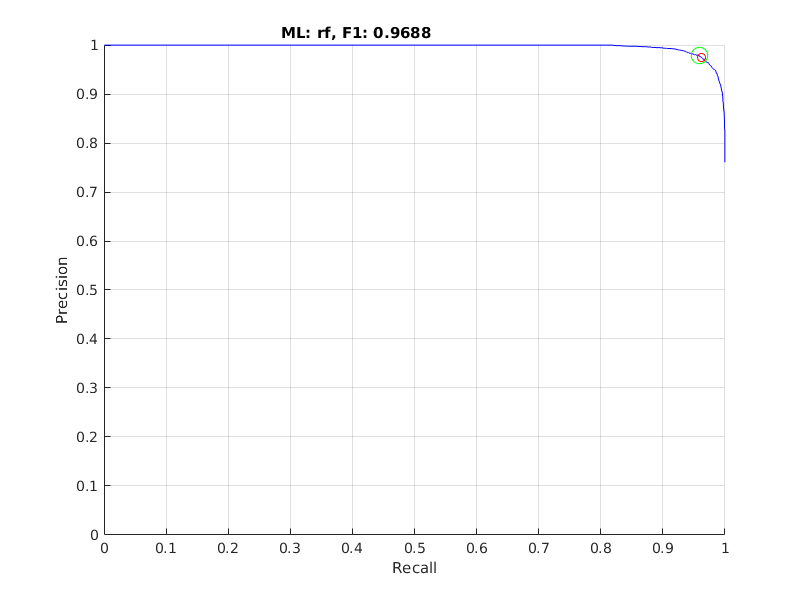
\includegraphics[width=0.95\linewidth]{./figures/siaf.png}
\end{center}
   \caption{}
\label{fig:siaf}
\end{figure}

\begin{figure}[t]
\begin{center}
   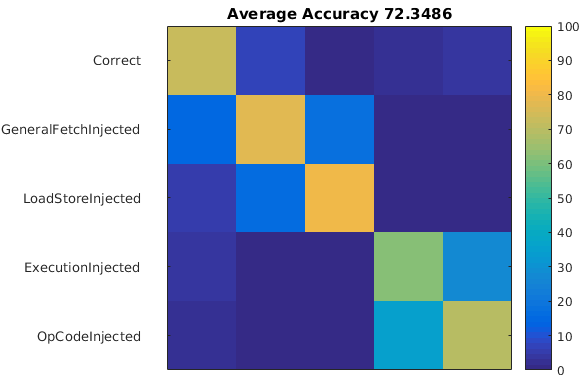
\includegraphics[width=0.95\linewidth]{./figures/siaf_multi.png}
\end{center}
   \caption{}
\label{fig:siaf-multi}
\end{figure}

\begin{figure}[t]
\begin{center}
   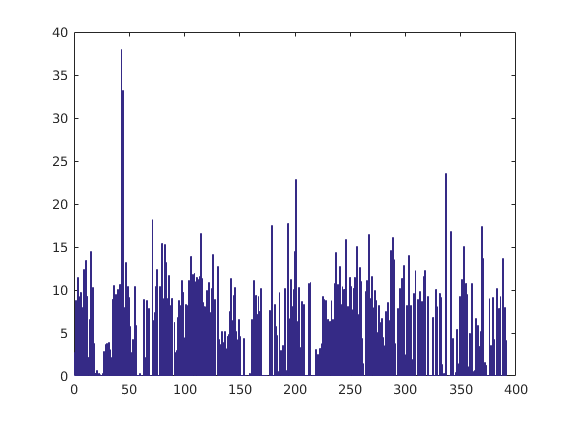
\includegraphics[width=0.95\linewidth]{./figures/feat_same.png}
\end{center}
   \caption{}
\label{fig:feat-same}
\end{figure}

\subsection{Same Input Different Features}

\begin{figure}[t]
\begin{center}
   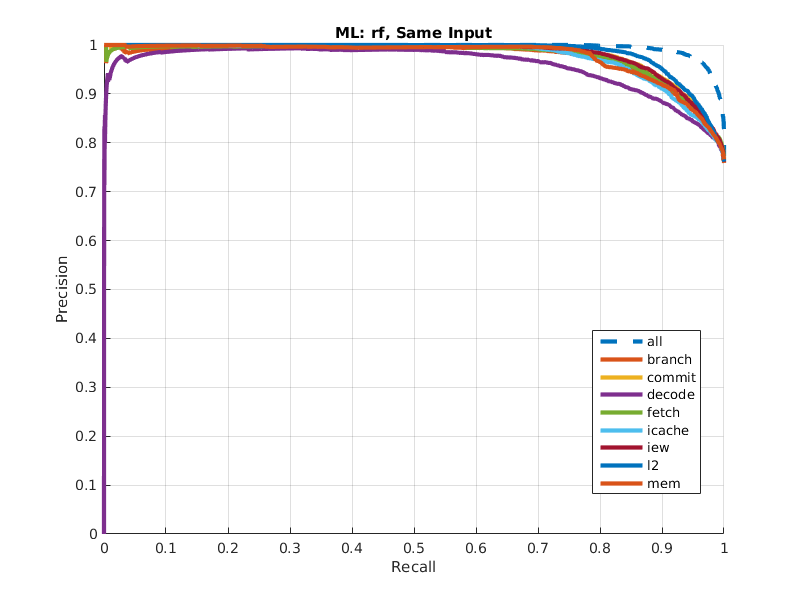
\includegraphics[width=0.95\linewidth]{./figures/sidf.png}
\end{center}
   \caption{}
\label{fig:sidf}
\end{figure}

\subsection{Different Input All Features}

\begin{figure}[t]
\begin{center}
   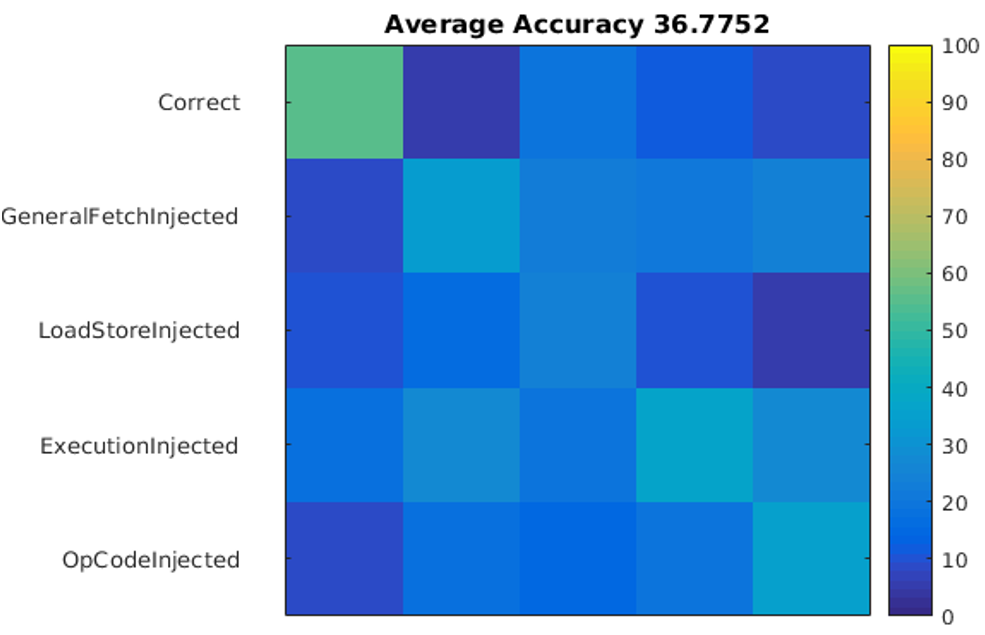
\includegraphics[width=0.95\linewidth]{./figures/diaf_multi.png}
\end{center}
   \caption{}
\label{fig:diaf-multi}
\end{figure}

\begin{figure}[t]
\begin{center}
   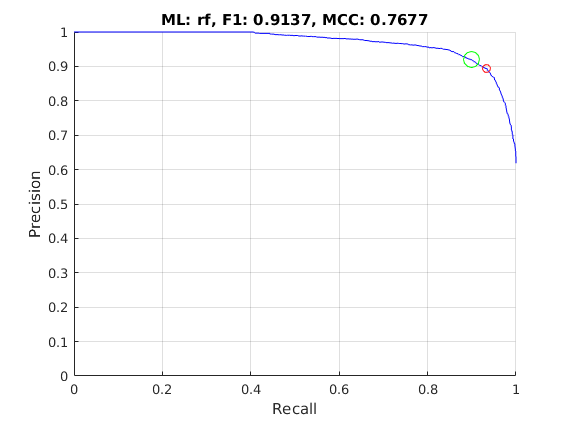
\includegraphics[width=0.95\linewidth]{./figures/disf.png}
\end{center}
   \caption{}
\label{fig:disf}
\end{figure}

\begin{figure}[t]
\begin{center}
   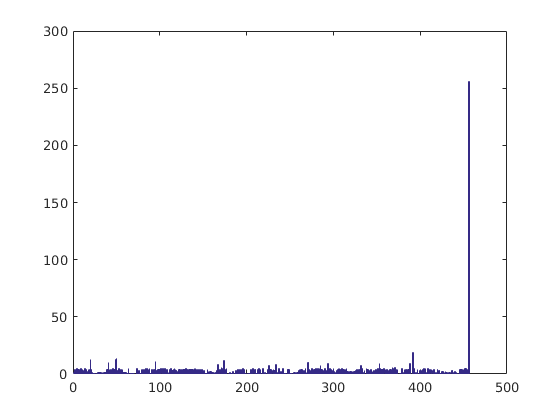
\includegraphics[width=0.95\linewidth]{./figures/feat_diff.png}
\end{center}
   \caption{}
\label{fig:feat-diff}
\end{figure}

\subsection{Different Input Different Features}

\begin{figure}[t]
\begin{center}
   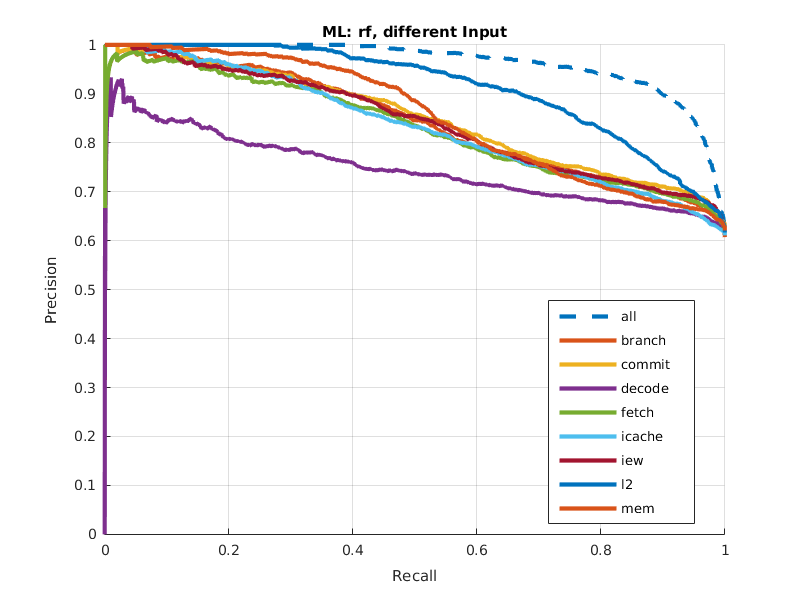
\includegraphics[width=0.95\linewidth]{./figures/didf.png}
\end{center}
   \caption{}
\label{fig:didf}
\end{figure}


\section{Discussion and Conclusion}
\cite{lamport94}

%%%%%%% -- PAPER CONTENT ENDS -- %%%%%%%%

%%%%%%%%% -- BIB STYLE AND FILE -- %%%%%%%%
\bibliographystyle{ieeetr}
\bibliography{ref}
%%%%%%%%%%%%%%%%%%%%%%%%%%%%%%%%%%%%

\end{document}
